% !TEX root = deplump.tex
\section{Algorithm}

\newcommand{\T}{\ensuremath{\mathcal{T}}}
\newcommand{\N}{\ensuremath{\mathcal{N}}}
\newcommand{\M}{\ensuremath{\mathcal{M}}}
\newcommand{\PP}{\ensuremath{\mathcal{P}}}
\newcommand{\nc}{\ensuremath{nc}}
\newcommand{\RS}{\ensuremath{\mathcal{R}\mathcal{S}}}
\newcommand{\D}{\ensuremath{\mathcal{D}}}
\newcommand{\la}{\ensuremath{\leftarrow}}
\newcommand{\G}{\ensuremath{\mathcal{G}}}
\newcommand{\IS}{\ensuremath{\mathcal{I}\mathcal{S}}}
\newcommand{\Seq}{\ensuremath{\mathcal{S}}}
\newcommand{\dd}{\ensuremath{\delta}}

\begin{figure*}[t] 
	\begin{center}
		\scalebox{.6}{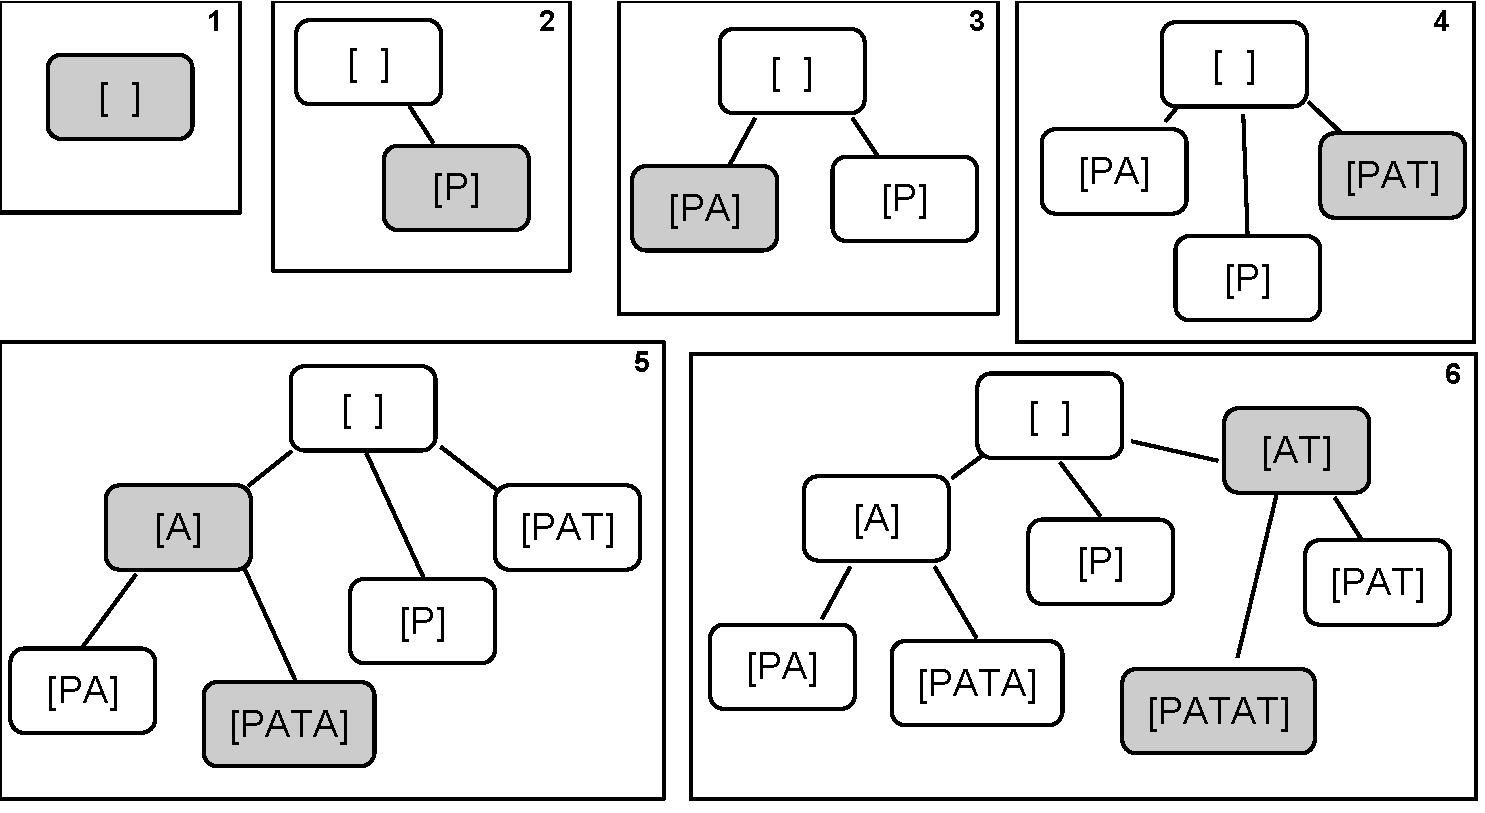
\includegraphics{figs/PATAT.pdf}} % [clip=true, viewport= 1in 1in 9in 9in]
		\caption{Construction of suffix tree for string ``PATAT".  In each frame the new nodes are shaded in gray.}
		\label{fig:suffix_tree}
	\end{center} 
\end{figure*} 

Given a sequence of symbols $[s_0, s_1, s_2, \ldots]= [\sigma_{101}, \sigma_3, \sigma_{17}, \ldots]$ where each symbol $s_n$ comes from from an ordered set of symbols $\{\sigma_0, \sigma_1, \ldots\} \in \Sigma$,  deplump works by repeatedly producing a predictive distribution for the continuation of the sequence given the full preceding context and encoding the next symbol by passing that predictive distribution to an entropy encoder.  
% (as most streaming, probabilistic, general-purpose lossless compression algorithms) 
%A discrete predictive distribution function is produced for each context and used encode the subsequent symbol. 
In this paper explicit details related to encoding and decoding are not included, instead we present the algorithms necessary to incrementally construct the predictive distributions needed by the encoder and decoder.  Specifically, we assume that if the predictive distribution function is $F$ and the next symbol in the stream is $s$ then the stream can be compressed using an entropy encoder that takes $F(s-1)$ and $F(s)$ as arguments and returns a bit stream (possibly null)\cite{rangeencoding,arithmeticencoding}.   The cumulative distribution function will always be well defined because we assume an ordering of the symbols, i.e.~the notation $s-1$ refers to the symbol prior to $s$ in the sequence of observed symbols.  Note that the symbol set can be ordered as the set is discovered.
%Decompression details are also omitted but is implemented as usual as in entropy encoder/decoder pairs .

%To decompress, the range decoder takes $F$ and the compressed stream as arguments and returns the next symbol in the uncompressed sequence. In the algorithm the functions RangeEncode() and RangeDecode() indicate these operations.   In order to decompress the stream the exact same predictive model will need to be built from the compressed stream.  This requires that the model estimate prior to compressing $s_n$ is a function of fixed parameters and the symbols $[s_0, s_1, \ldots, s_{n-1}]$ because those are the only symbols available to the decompressor for decompressing $s_n$.  

Deplump consists of a set of recursive algorithms run over an incrementally constructed suffix-tree-like datastructure \citep{Ukkonen1992}.  %A suffix tree is a data structure for keeping track of the unique suffices in a set of strings.  The tree structure arranges the suffices hierarchically which makes it easy to search.  
This datastructure efficiently encodes the set of all predictive contexts in a sequence (i.e.~the set $\{ [ ], [s_0], [s_0,s_1], [s_0, s_1,s_2], \ldots \}$).   Every node in the tree corresponds to a unique predictive context.  Each node in the tree is indexed by a sequence of symbols $[s_m, \ldots, s_{m + k}]$ (note that a node is looked up by traversing edges in the tree that match the sequence of symbols one gets from reading this sequence right to left).  We use $\N$ to interchangeably refer to a node and the context to which the node corresponds. An edge between two nodes in the tree will in general be labeled with a sequence of symbols of length greater than or equal to one.  Deplump incrementally constructs this this tree is handled by the function CreateNode($\N, \M$) makes the creation of node $\N$ with parent $\M$ explicit. The parent of node $\N$ is referenced as ${Pa}(\N)$.

Each node instance $\N$ contains two counts for each $s \in \Sigma$, $c_s$ and $t_s$.  We use $c$ and $t$ to refer to the marginal counts $\sum_{s \in \Sigma} c_s$ and $\sum_{s \in \Sigma} t_s$.  Each node also has a discount $d$ associated with it.  The discount associated with $\N$ is a function of $\D$ (the discount parameters of the model), $|\N|$, and $|$PA$(\N)|$.  The discount for $\N$ is calculated by GetDiscount(\N). Suffix tree data structures use a reference sequence (\RS) to store the unique suffices in the tree.  Therefore, each node instance also contains two indices related to $\RS$ from which the context specific to that node can be reconstructed.  If the indices for $\N$ are $i$ and $j$, then the context associated with $\N$ is $\RS[i : j]$.

The reference sequence grows with the length of the input sequence and must be shortened as the algorithm progresses.  The shortening of $\RS$ is made explicit by the $\sigma$ function in CDFNextSymbol.  The function $\sigma(\Seq)$ returns $\Seq[2:$end$]$.  When $\RS$ is shortened, nodes in the suffix tree which reference removed sections are no longer usable and must be removed from the tree to prevent a memory leak.  To facilitate the removal process pointers are maintained from the elements of $\RS$ to the suffix tree nodes which reference them.  Without the use of pointers, deletion of the unusable nodes requires a search over the tree which is prohibitive for large trees. The cost of these operations can be amortized by shorting $\RS$ in chunks and keeping pointers from each chunk of $\RS$ instead of each element.  To minimize the impact of rendering nodes unusable by shortening the reference sequence, suffix tree nodes are updated as the algorithm progresses to reference recent sections of $\RS$.


%The reference sequence $\RS$ is implemented as a linked list. Therefore, instead of using a simple $i,j$ index in each suffix tree node, $i$ is replaced by a linked list node and an offset and $j$ is replaced by a string length $l$.  Each node of the linked list must contain a list of suffix tree nodes which reference it.  The reference sequence grows as the length of the input sequence grows and must be shortened as the algorithm progresses.  The shortening of $\RS$ is made explicit by the $\sigma$ operator in CDFNextSymbol, which returns the argument sequence shortened by removing the fist element.  When $\RS$ is shortened, nodes in the suffix tree which reference removed sections are no longer usable and must be removed from the tree to prevent a memory leak.  Without a list of suffix tree nodes which reference each linked list node, deletion of the unusable nodes requires a search over the tree which is prohibitive for large trees.  The cost of these operations can be amortized by shorting $\RS$ in chunks, i.e. by removing nodes of the linked list.  To minimize the impact of rendering nodes unusable by shortening the reference sequence, nodes should be updated to point to the most recent part of $\RS$ as possible.

Several parameters required by the model must be assigned at initialization.  They are $\D$, $k$, $L$, $\eta$,  and depth.  $\D = [\dd_0, \dd_1, \ldots, \dd_{10}, \alpha]$ is a list of discount parameters, each taking a real value in $(0,1)$.  The parameter $k$ is positive integer valued and is an upper bound on the total count $c$ in each node.  The parameter $L$ is an upper bound on the number of node instances in the suffix tree.  We use $100L$ as an upper bound on the length of $\RS$, but there is no explicit reason to tie these two upper bounds together. The parameter $\eta$ is a learning rate for the updating of the discount parameters and is typically set very small.  Finally, the depth of the tree can be limited by a positive integer.  Depth is not considered in Algorithm~\ref{alg}, but it could be incorporated into the function GetNode.

Since the model must be estimated incrementally, the suffix tree must also be incrementally constructed.  Construction of the tree is handled by the function GetNode and FragmentNode in Algorithm~\ref{alg}.  An illustration of the incremental construction can be seen in Figure~\ref{fig:suffix_tree} for the toy sequence [PATAT].   In frame 4 the function GetNode assigns [ ]  to $\M$ and then [PAT] to $\Seq$ with $\M = $ PA$(\Seq)$. In Frame 5 GetNode assigns [PA] to $\M$, but then must assign [A] = FragmentNode(\M) to $\PP$ and PA$(\M)$ to \PP.  Node $\Seq$ is then created by CreateNode$($[PATA]$,\PP)$.  In each frame the first step is to find $\M$, which can be achieved by descending an appropriate path of the suffix tree.  All of the nodes on the path to $\M$ and possibly $\M$ itself can have the indices into $\RS$ updated to point to a more recent section of the reference sequence. 

For each $s$ in the input sequence the function PMFNextSymbol is called to obtain the predictive probability mass function (PMF).  The function PMFNextSymbol enforces the upper bounds on $|\RS|$ and $nc$.  If  $|\RS|$ is hitting the upper bound then then $\RS$ is shortened as described, if $nc$ is hitting the upper bound then leaf nodes of the suffix tree are deleted uniformly at random.  Note that the deleting of leaf nodes uniformly at random is non-trivial to implement. One approach is to maintain an active list must of all the leaf nodes throughout the algorithm. A second approach is for each node to maintain a count of thenumber of leaf nodes in the subtree beneath it.  Given that each node contains the exact number of leaf nodes beneath it a random leaf node can be obtained by taking a weighted random path down the tree.  Finally, PMFNexSymbol returns the predictive PMF.

    After encoding or decoding using the predictive PMF $pi$ the first step in updating the model estimate is performed by the function UpdateCountsAndDiscounts.  Starting at node $\N$ and progressing up to the root of the tree, $c_s$ is incremented if $t_s$ was incremented in the node below.  If $c_s$ is incremented, a stochastic decision is made to increment $t_s$.  The gradients for the discount parameters $\D$ are updated by the function UpdateDiscountParameterGradients.  If $c$ is larger than $k$ in any of the nodes, the counts $c_s$ and potentially $t_s$ are reduced by the function ThinCounts. Finally, \D \space is updated based on the calculated gradients and the specified learning rate $\eta$ and the symbol is appended to \RS.


\begin{algorithm}
    \caption{Deplump} \label{alg}
    \begin{algorithmic}[1]
    
    	\Procedure{Deplump/Plump}{$\IS$}
		\State $\RS \la [$ $]  $ \Comment{reference sequence}
		\State Initialize $[$ $]$ node of \T \Comment{suffix tree}
		\State $\nc \la 1$ \Comment{node count}
		\State $\D \la  \{ \dd_0, \dd_1, \dd_2, \dots, \dd_{10}, \alpha \}$ \Comment{discount parameters}
		\State $\G \la \vec 0$ \Comment{discount parameter gradients, $|\G| = |\D|$}
		\State $\mathcal{O}\mathcal{S} \la  [$ $]$ \Comment{output sequence}
		\For{i = 1: $| \IS|$}
			\State [$\pi$, \N] $\la$ PMFNextSymbol(\RS)
			\If{Plump}
				\State $s \la $ RangeDecode($\pi$, \IS)
				\State $\mathcal{O}\mathcal{S} \la [\mathcal{O}\mathcal{S}$ $s]$
			\Else
				\State $s \la \IS[i]$
				\State $b \la$ RangeEncode$(\Sigma_{i = 1}^{s-1} \pi_i, \Sigma_{i = 1}^{s} \pi_i$)
				\State $\mathcal{O}\mathcal{S} \la [\mathcal{O}\mathcal{S}$ $b]$		
			\EndIf
			\State UpdateCountsAndDiscountGradients($\N,s,\pi_s,$TRUE)
			\State $\D \la \D + \G \eta / (\pi_s)$ \Comment{update discount parameters}
			\State $\G \la \vec 0$ \Comment{reset gradients to zero}
			\State $\RS \la [\RS$ $s]$ \Comment{append symbol to reference sequence}
		\EndFor
		\State \Return $\mathcal{O}\mathcal{S}$
	\EndProcedure
	
	\Function{PMFNextSymbol}{$\RS$}
		\While{$ |\RS| \geq 100 L$}
			\State Delete nodes referencing \RS[1] and update $nc$
			\State $\RS \la \sigma(\RS)$
		\EndWhile
		\While{ $\nc > (L - 2)$}
			\State Delete leaf node uniformly at random
			\State $nc \la nc -1$
		\EndWhile
		
		\State $\N \la$ GetNode$(\RS, \T)$
		\State $\pi \la$ PMF($\N, \vec 0, 1.0$) \Comment{$| \vec 0| = | \Sigma|$}
	%	\State UpdateCountsAndDiscountGradients($\N,s,\pi_s,$TRUE)
		\State \Return [$\pi$, \N]
	\EndFunction
	
	
	 \end{algorithmic}
\end{algorithm}

\begin{algorithm}
    \caption{Deplump Continued}
    \begin{algorithmic}[1]
    

%    	\Function{PointOnCDFNextSymbol}{$h,\T,\RS$}
%		\While{$ |\RS| \geq 100 L$}
%			\State Delete nodes referencing \RS[0]
%			\State $\RS \la \sigma(\RS)$
%		\EndWhile
%		\While{ $\nc > (L - 2)$}
%			\State Delete leaf node uniformly at random
%		\EndWhile

%		\State $\N \la$ GetNode$(\RS, \T)$
%		\State $\pi \la$ PMF($\N, \vec 0, 1.0$) \Comment{$| \vec 0| = | \Sigma|$}
%		
%		\State $F(s) \la 0$
%		\State $s \la 0$
%		\While{$F(s) < h$}
%			\State $s \la s + 1$
%			\State $F(s) \la F(s) + \pi_s$
%		\EndWhile
%		
%		\State $F(s-1) \la F(s) - \pi_s$
%		\State Update $h$
%		\Return  $[h,s, F(s-1), F(s)]$
%	\EndFunction
	
	\Function{GetDiscount}{\N}
		\State $d = 1.0$
		\If{\N = [ ]}
			\State \Return $\dd_0$
		\EndIf
		\For{$i = (|$PA$(\N)| + 1): |\N|$}
			\If{$i \leq 10$}
				\State $d \la d \delta_i$ \Comment{multiply by discount parameter $i$}
			\Else
				\State $d \la d \dd_{10}^{\alpha^i}$
			\EndIf
		\EndFor
		\State \Return $d$
	\EndFunction
    
    	\Function{GetNode}{\Seq, \T}
		\State Find the node \M \space in the suffix tree sharing the longest suffix with \Seq.
		\If{\M \space is a suffix of \Seq}
			\If{$\Seq = \M$}
				\State \Return \M
			\Else
				\State $\Seq \la$ CreateNode$(\Seq, \M)$
				\State $nc \la nc + 1$
				\State \Return \Seq
			\EndIf
		\Else
			\State \PP \la \space FragmentNode(\M, \Seq)
%			\State PA(\M) \la \space \PP
			\State $\Seq \la $ CreateNode$(\Seq, \PP)$
			\State $nc \la nc + 1$
			\State \Return \Seq
		\EndIf
	\EndFunction
    
    	    \end{algorithmic}
\end{algorithm}

\begin{algorithm}
	\begin{algorithmic}[1]
	\caption{Deplump Continued}
	
	\Function{UpdateCountsAndDiscounts}{$\N, s, p$, BackOff}
		\State $d \la $ GetDiscount(\N)
		\State $pp \la p$
		\If{$c > 0$}
			\State $pp \la (p - \frac{c_s - t_s d}{c}))(\frac{c}{t d})$
			\State $w \la c_s	+ d(t *pp - t_s)$		
		\EndIf
		
		\If{BackOff  and $c > 0$}
			\State $c_s \la c_s + 1$
			\State BackOff $\la 0$
			\State BackOff $\la 1$ w.p. $pp (\frac{t d}{w})$ \Comment{w.p abbreviates ``with probability"}
			\If{BackOff}
				\State $t_s \la t_s + 1$
			 \EndIf
		\ElsIf{BackOff}
				\State $c_s \la c_s + 1$
				\State $t_s \la t_s + 1$
		\EndIf
		\State UpdateDiscountParameterGradients($t_s, t,pp, d$)
		\State UpdateCountsAndDiscounts(PA(\N), $s,pp$, BackOff)
		\State ThinCounts(\N)
	\EndFunction
			
	\Function{ThinCounts}{$\N$}
		\State $d \la$ GetDiscount$(\N)$
		\While{$c > k$}
			\State $s \la $ DrawMultinomial$(\pi)$ s.t. $\pi_l = \frac{c_l}{c}$ \Comment{$\pi$ is a distribution over $\Sigma$}
			\State $\phi \la$ SamplePartition$(c_s, t_s, d)$
			\State $i \la$ DrawMultinomial$([\frac{\phi_1}{c_s}, \frac{\phi_2}{c_s}, \ldots, \frac{\phi_{t_s }}{c_s} ])$
			\If{$\phi_i == 1$}
				\State $t_s \la t_s - 1$
			\EndIf
			\State $c_s \la c_s - 1$
		\EndWhile
	\EndFunction	
	
	\end{algorithmic}	
\end{algorithm}

\begin{algorithm}
	\begin{algorithmic}[1]
	\caption{Deplump Continued}

\Function{PMF}{$\N, \pi, m$}
		\State $d \la $ GetDiscount(\N)		
		\If{$c > 0$}
			\For{$s \in \Sigma$}
				\State $\pi_s\la \pi_s + m(\frac{c_s - t_s d}{c})$
			\EndFor
		\EndIf
		
		\If{PA$(\N) \neq$ null}
			\State \Return PMF(PA(\N), $\pi, d m$)
		\Else
			\State $\pi \la (1- d m)\pi + dm\mathcal{U}(\Sigma)$ \Comment{$\mathcal{U}(\Sigma)$ is the uniform distribution over $\Sigma$}
			\State \Return $\pi$
		\EndIf 
	\EndFunction
	
	\Function{FragmentNode}{$\M, \Seq$}
		\State $d^\M \la$ GetDiscount(\M)
		\State $\PP \la$ maximum overlapping suffix  of \M \space and \Seq
		\State $\PP \la $ CreateNode$(\PP,$ PA$(\M))$
		\State $nc \la nc + 1$
		\State PA(\M) $\la \PP$
		\State $d^\PP \la$ GetDiscount(\PP)
		\For{$s \in \Sigma$}
			\State $\phi \la$ SamplePartition $(c^\M_s, t^\M_s,d^\M)$
			\State $t^\PP_s \la t^\M_s$
			\State $t^\M_s \la 0$
			\For{$i= 1 : | \phi|$}
				\State $a \la$ DrawCRP$(\phi[i],d^\M / d^\PP,-d^\M)$
				\State $t_s^\M \la t_s^\M + a$
			\EndFor
			\State $c^\PP_s \la t^\M_s$
		\EndFor
		\State \Return \PP
	\EndFunction
	
	\Function{DrawCRP}{$n,d,c$} \Comment{$ n \geq 1$}
		\State $t \la 1$
		\For{i = 2 : n}
			\State $r \la 0$
			\State $r  \la 1$ w.p. $\frac{td + c}{i-1 + c}$
			\State $t \la t + r$
		\EndFor
		\State \Return $t$
	\EndFunction
	
	\end{algorithmic}	
\end{algorithm}

\begin{algorithm}
	\begin{algorithmic}[1]
	\caption{Deplump Continued}
	
	\Function{SamplePartition}{$c,t,d$}
		\State $M \la  t \times c$ matrix of zeros
		\State $M(t,c) \la 1.0$
		\For{$j = (c-1) : 1$}
			\For{$i = 1 : (t-1)$} 
				\State $M(i,j) \la M(i +1, j+1) + M(i,j+1)(j - id)$ 
			\EndFor
			\State $M(d,j) \la M(t,j+1)$
		\EndFor
		\State $\phi \la \vec 0$ \Comment{$|\vec 0| = t$}
		\State $\phi[1] \la 1$
		\State $k \la 1$
		\For{j = 2 : c}
			\State $M(k,j) \la M(k,j)(j-1 -k d)$
			\State $r \la 0$
			\State $r \la 1 $ w.p. $\frac{M(k+1,j)}{M(k+1,j) + M(k,j)}$
			\If{r = 1}
				\State $k \la k + 1$
				\State $\phi[k]  \la 1$
			\Else
				\State $i \la$ DrawMultinomial$([\frac{\phi[1] - d}{j-1 -kd}, \frac{\phi[2] - d}{j-1 -kd}, \ldots, \frac{\phi[k] - d}{j-1 -kd}])$
				\State $\phi[i] \la \phi[i] + 1$
			\EndIf
		\EndFor
		\State \Return $\phi$
	\EndFunction

	\Function{UpdateDiscountParameterGradients}{$\N, t_s, c, t, pp, d, m$}
		\If{$c > 0$}
			\If{$|\N| = 0$}
				\State $ \psi \la \frac{1.0}{\dd_0}$
				\State $\G_0 \la \G_0 + (d(t * pp - t_s)\psi / c)  m$
			\Else
				\State $z \la |$PA(\N)$| + 1$
				\While{$z \leq |\N|$ and $z < 10$}
					\State $\psi \la \frac{1.0}{\dd_z}$
					\State $\G_z \la \G_z + (d(t * pp - t_s) \psi / c)  m$	
				\EndWhile
				
				\If{$|\N| \geq 10$}
					\State $a \la z - 10$
					\State $b \la |\N| - z + 1$
					\State $\psi \la \alpha^a(1 - \alpha^b) / ((1 - \alpha)  \dd_{10})$ 
					\State $\G_{10} \la \G_{10} + (d(t * pp - t_s) \psi / c)  m$	
					\State $\psi \la$ log$(\dd_{10}) (a \alpha^{a-1} - (a + b)\alpha^{a + b-1}) / (1 - \alpha) + (\alpha^a - \alpha^{a + b}) / (1 - \alpha)^2$
					\State $\G_{11} \la \G_{11} + (d(t * pp - t_s)\psi / c)  m$	
				\EndIf
			\EndIf
		\EndIf
	\EndFunction

	\end{algorithmic}	
\end{algorithm}

